% ==============================================================================
% Plantilla Institucional de Trabajo Terminal — UPIIZ IPN
% Archivo: apendices/protocolo-anexo.tex
% ==============================================================================
% ANEXOS INSTITUCIONALES PARA EL MODO PROTOCOLO:
% Conforme a los puntos 17 y 18 del Anexo 1 del Reglamento de Trabajo Terminal:
% - 17. Currículum Vitae (CV) de los asesores (resumido, máx. 2 páginas por asesor).
% - 18. Anexo 2: Instrumento de Evaluación de Protocolo (última hoja reglamentaria).
% ==============================================================================

\clearpage
\pagestyle{empty}

% Registro en el Índice general
\phantomsection
\addcontentsline{toc}{chapter}{Anexo}

\begin{center}
    \vspace*{1.5cm}
    {\fontsize{18}{22}\bfseries\sffamily Anexo}\\[1.5em]
    {\fontsize{14}{18}\bfseries\sffamily Currículum Vitae (CV)}\\[2.0em]
\end{center}
\vspace{1.5cm}

% ------------------------------------------------------------------------------
% INCLUSIÓN DE ARCHIVOS PDF DE CV DE ASESORES
% ------------------------------------------------------------------------------
% Coloque los archivos en la carpeta "anexos/":
% - anexos/cv-asesor-1.pdf
% - anexos/cv-asesor-2.pdf (si existe segundo asesor)
% - anexos/cv-asesor-3.pdf (si existe tercer asesor)
% Si los archivos existen físicamente, se insertan automáticamente con \includepdf.

\IfFileExists{anexos/cv_rafa.pdf}{%
    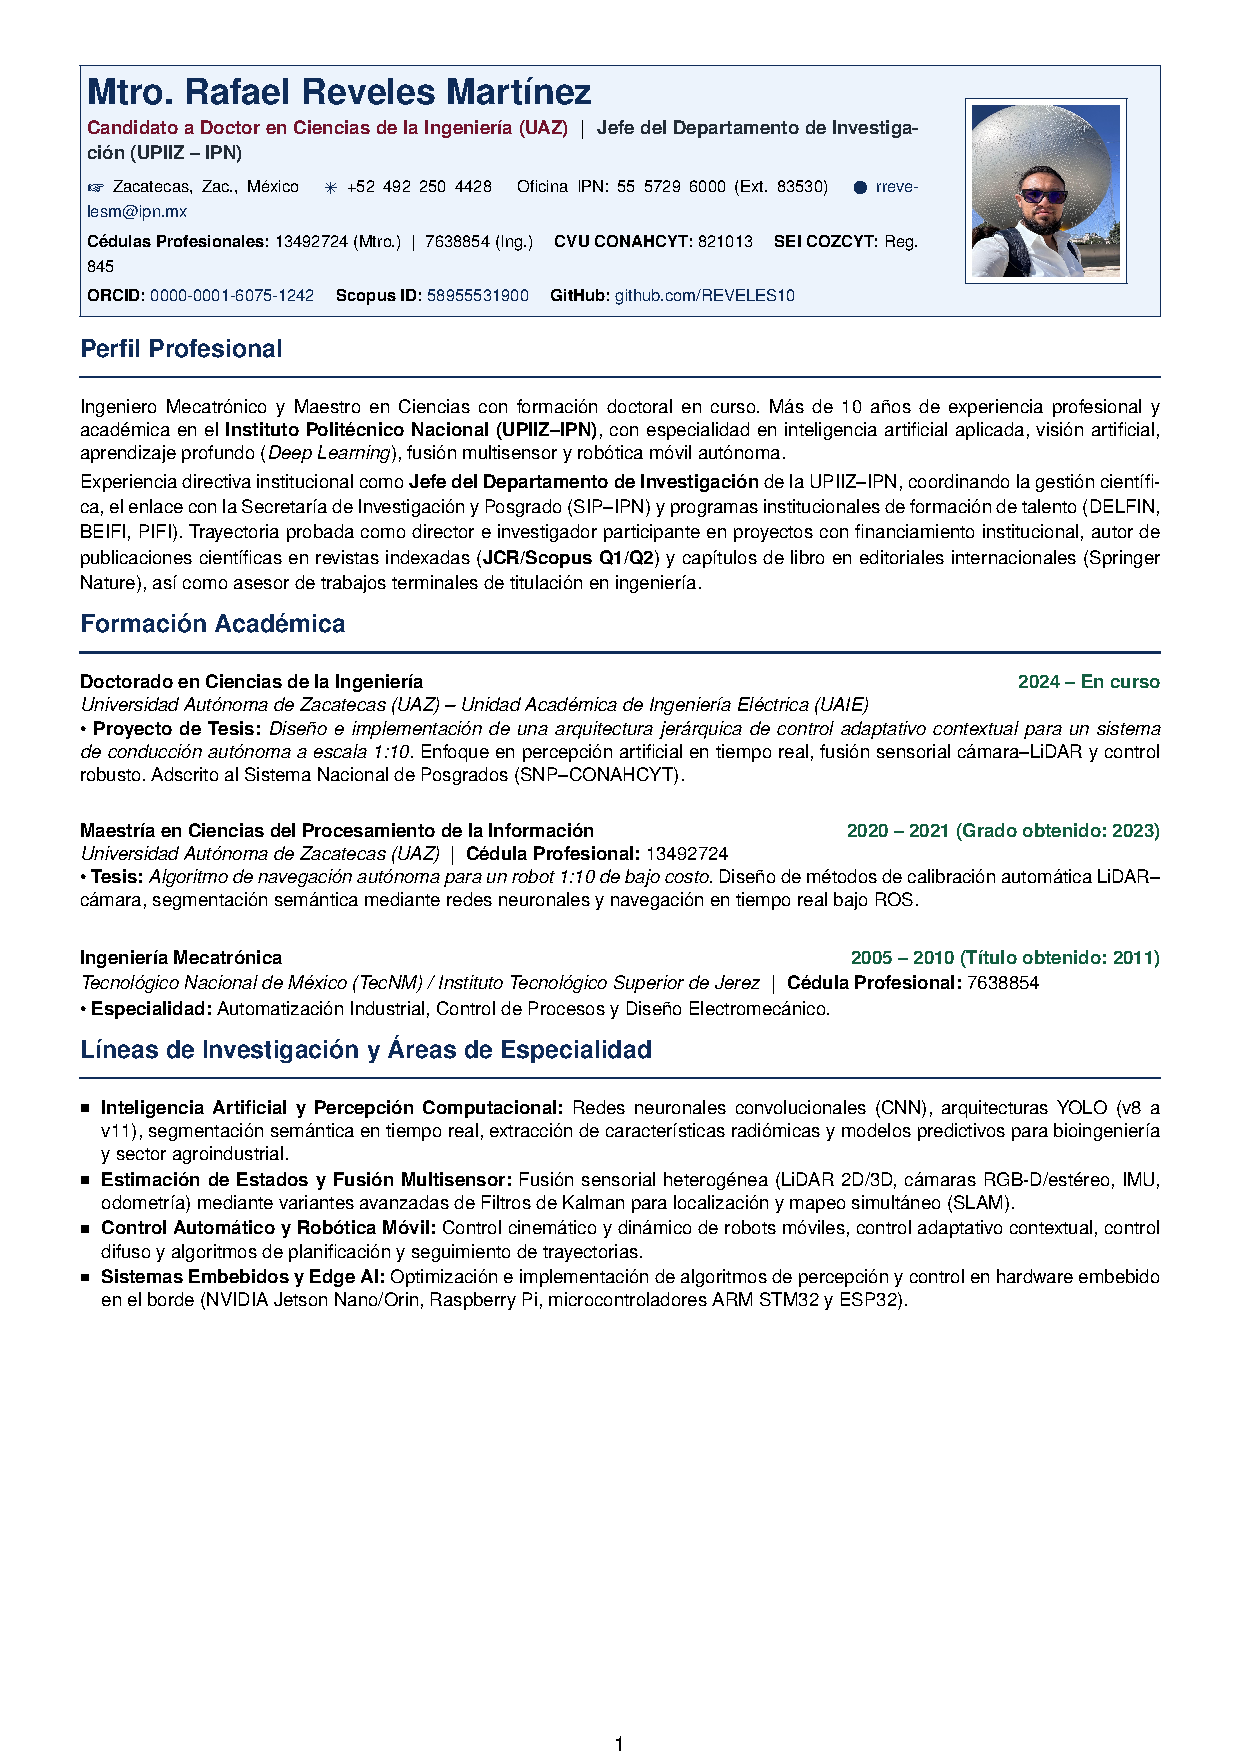
\includepdf[pages=1-2,pagecommand={\thispagestyle{empty}}]{anexos/cv_rafa.pdf}%
}{%
    \begin{center}
        \fbox{\parbox{0.88\textwidth}{%
            \centering\vspace{0.8em}
            \textbf{[Espacio para CV Resumido del Primer Asesor: \asesorANombre]}\\[0.4em]
            \small Deposite el archivo PDF en \texttt{anexos/cv-asesor-1.pdf} (máximo 2 páginas indicando cédula profesional).\\[0.8em]
        }}
    \end{center}
    \vspace{0.8cm}
}

\ifcsvoid{asesorBNombre}{}{%
    \IfFileExists{anexos/cv_sergio.pdf}{%
        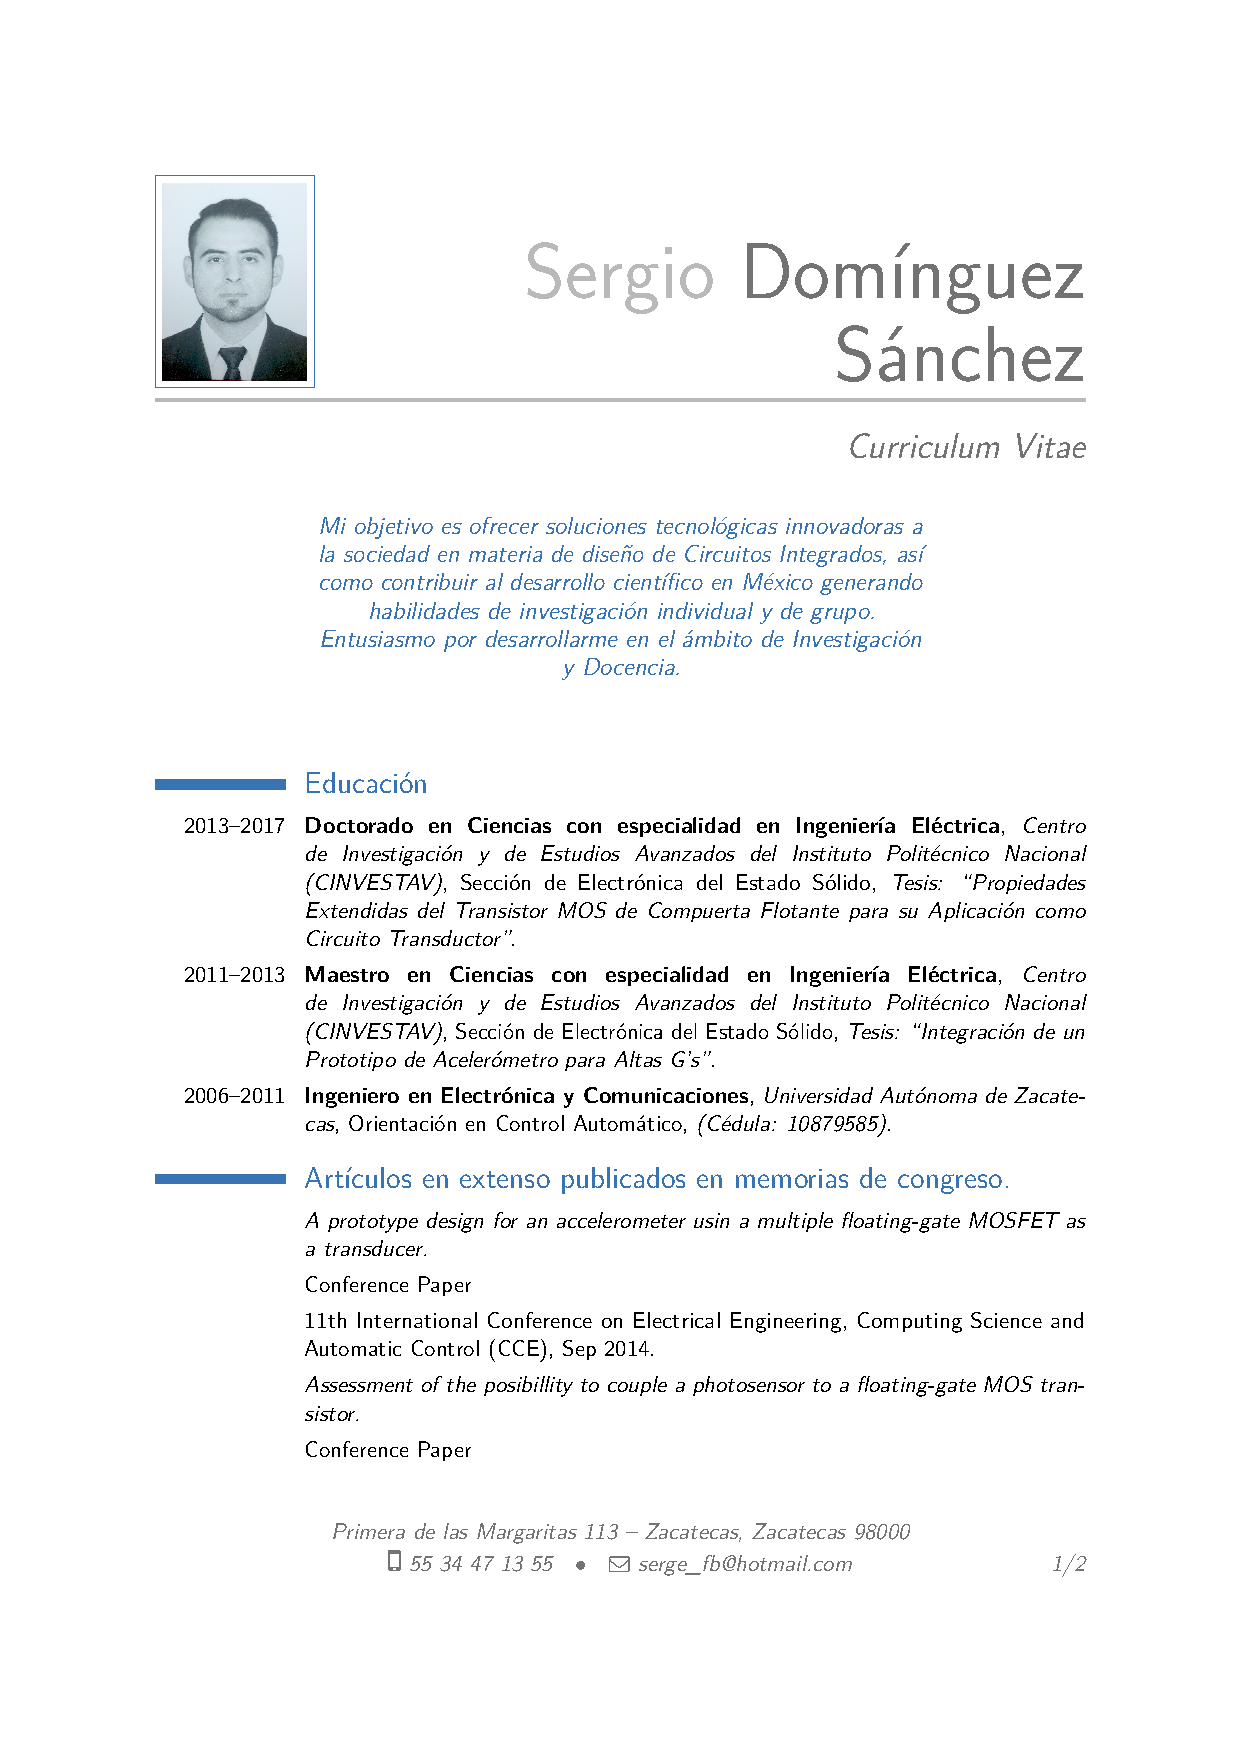
\includepdf[pages=1-2,pagecommand={\thispagestyle{empty}}]{anexos/cv_sergio.pdf}%
    }{%
        \begin{center}
            \fbox{\parbox{0.88\textwidth}{%
                \centering\vspace{0.8em}
                \textbf{[Espacio para CV Resumido del Segundo Asesor: \asesorBNombre]}\\[0.4em]
                \small Deposite el archivo PDF en \texttt{anexos/cv-asesor-2.pdf} (máximo 2 páginas indicando cédula profesional).\\[0.8em]
            }}
        \end{center}
        \vspace{0.8cm}
    }%
}

\ifcsvoid{asesorCNombre}{}{%
    \IfFileExists{anexos/cv_tala.pdf}{%
            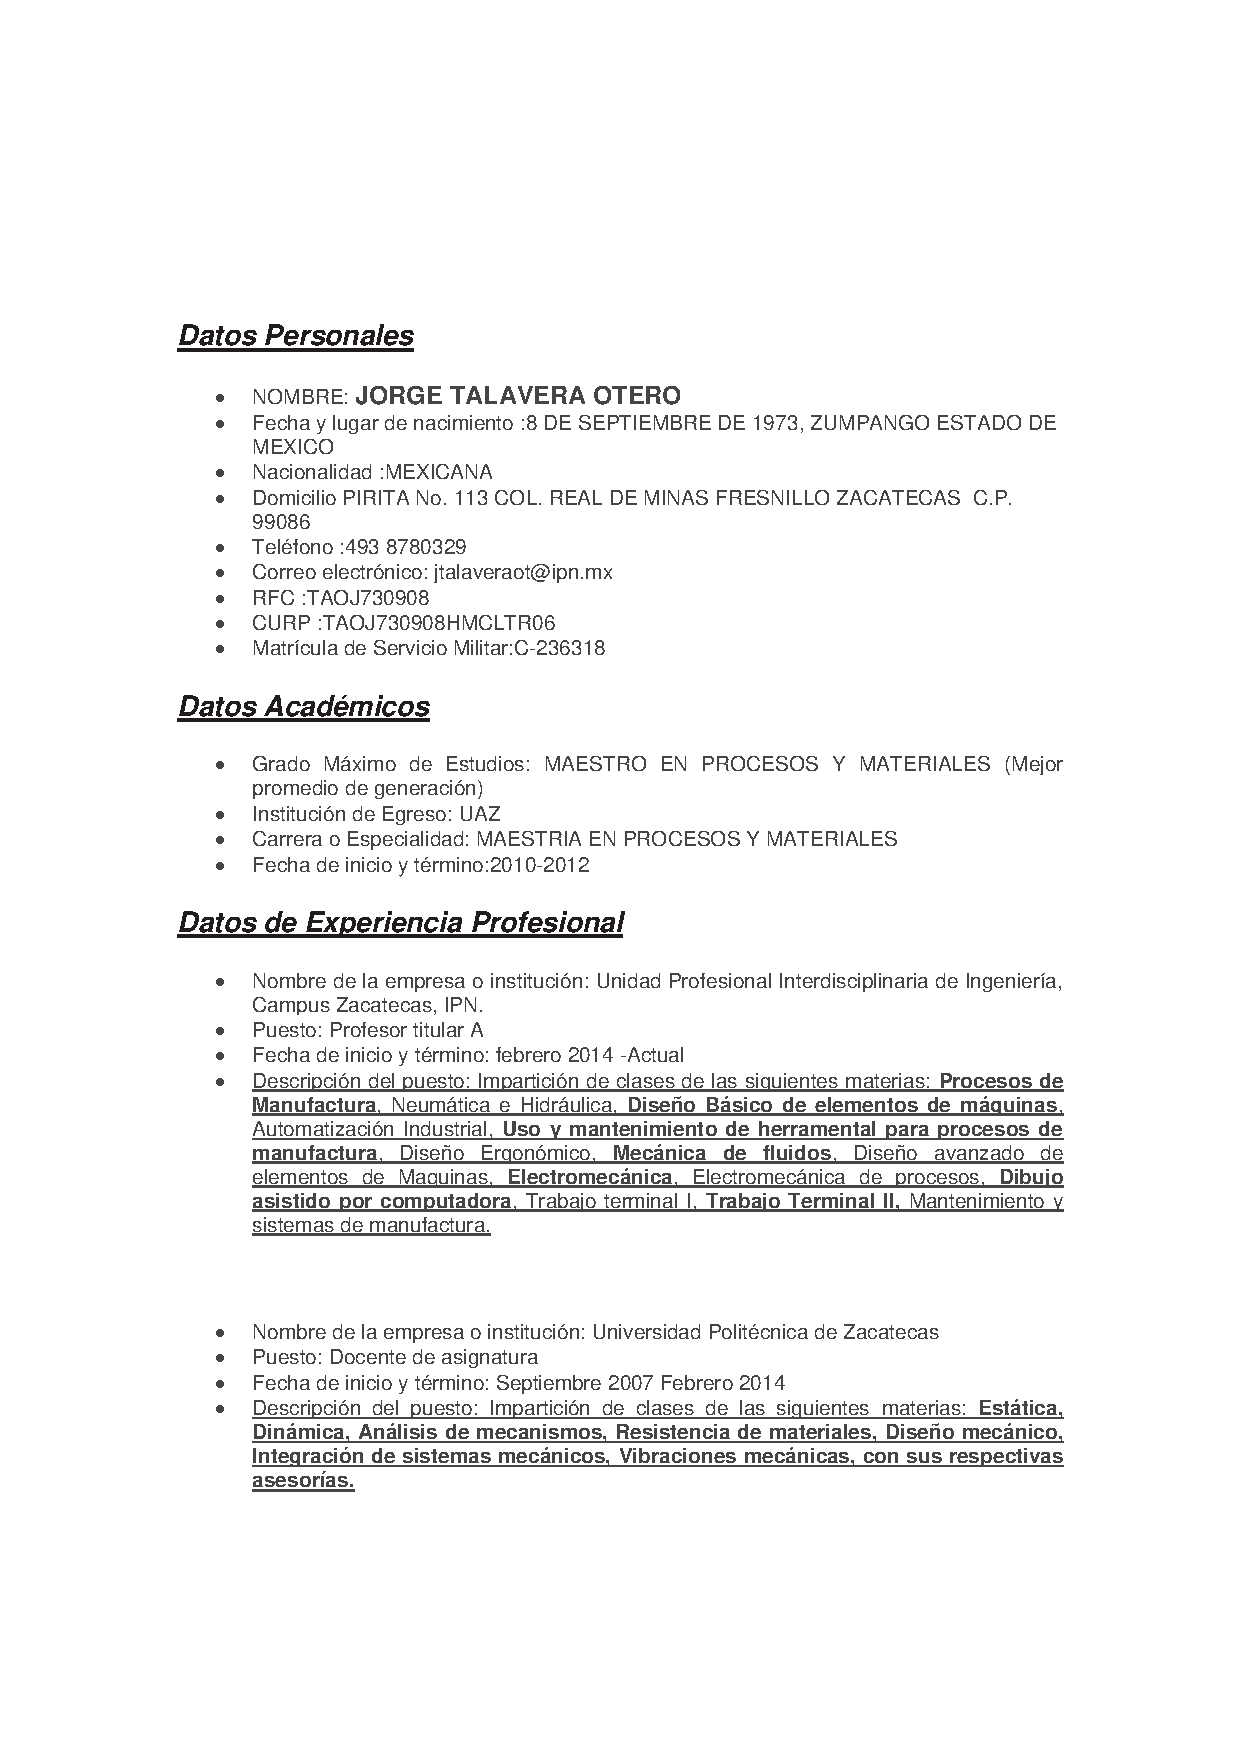
\includepdf[pages=1-2,pagecommand={\thispagestyle{empty}}]{anexos/cv_tala.pdf}%
    }{%
        \begin{center}
            \fbox{\parbox{0.88\textwidth}{%
                \centering\vspace{0.8em}
                \textbf{[Espacio para CV Resumido del Tercer Asesor: \asesorCNombre]}\\[0.4em]
                \small Deposite el archivo PDF en \texttt{anexos/cv-asesor-3.pdf} (máximo 2 páginas indicando cédula profesional).\\[0.8em]
            }}
        \end{center}
        \vspace{0.8cm}
    }%
}

% ------------------------------------------------------------------------------
% ÚLTIMA HOJA INSTITUCIONAL: ANEXO 2 (INSTRUMENTO DE EVALUACIÓN DE PROTOCOLO)
% ------------------------------------------------------------------------------
% El punto 18 del Anexo 1 establece que la última hoja del protocolo corresponderá
% al Anexo 2 del Reglamento para la evaluación de la Comisión Evaluadora.
% Coloque el archivo en "anexos/anexo-2-evaluacion.pdf" para su inclusión automática.

\IfFileExists{anexos/anexo_2.pdf}{%
    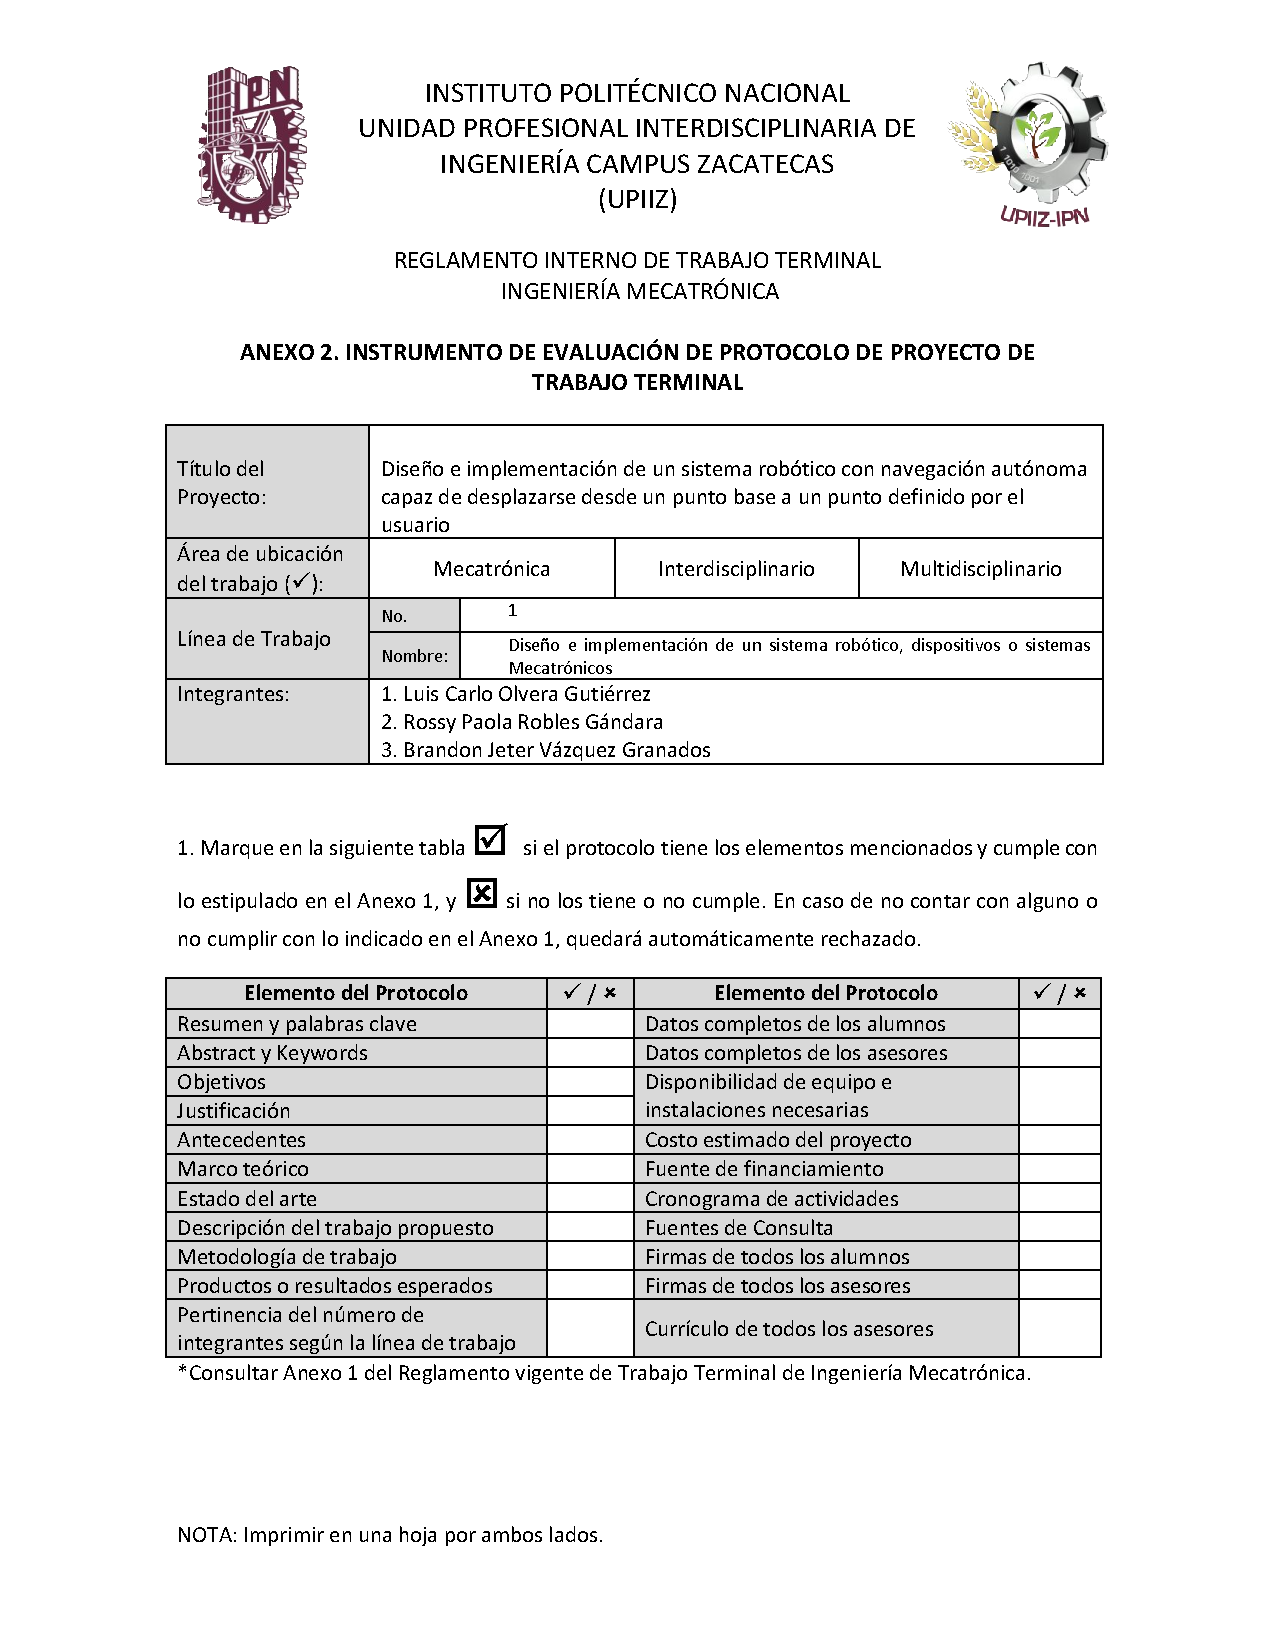
\includepdf[pages=1-3,pagecommand={\thispagestyle{empty}}]{anexos/anexo_2.pdf}%
}{%
    \vfill
    \begin{center}
        \fbox{\parbox{0.88\textwidth}{%
            \centering\vspace{0.8em}
            \textbf{[Última Hoja Institucional: Anexo 2 - Instrumento de Evaluación de Protocolo]}\\[0.4em]
            \small Para la entrega final, incorpore el formato oficial en \texttt{anexos/anexo-2-evaluacion.pdf} para que se anexe como la última hoja de acuerdo con el punto 18 del Anexo 1.\\[0.8em]
        }}
    \end{center}
    \vfill
}
